\documentclass{article}
\usepackage[utf8]{inputenc}
\usepackage{indentfirst} % to have indent in the first paragraphs
\usepackage{geometry}
\geometry{
    a4paper,
    left=30mm,
    right=30mm,
    top=20mm,
    bottom=25mm,
}
\renewcommand{\baselinestretch}{1.5}
\usepackage{times}
\usepackage{latexsym}
\usepackage{float}
\usepackage{graphicx}
\usepackage{microtype}
\usepackage{hyperref}
\usepackage{amssymb}
\usepackage{amsmath}
\usepackage[makeroom]{cancel}
\usepackage{import}
\usepackage{xcolor}
% \usepackage{tikz}
\usepackage{filecontents}
\usepackage{adjustbox}

\usepackage[backend=biber, style=alphabetic, sorting=ynt]{biblatex}
\addbibresource{bibliography.bib}

\title{IN-STK5000 - Project 2b - Fairness}
\author{Aurora Poggi, Fábio Rodrigues Pereira, Nick Walker \\
\emph{Project 9}}
\date{November 2021}

\begin{document}

\maketitle

\tableofcontents

\clearpage

\section{Introduction}
\label{sec: Introduction}

%What is fairness
In this document, we investigate the Covid-19 vaccination policy and decision making process we have designed previously in order to determine: 
\begin{itemize}
    \item Whether the policy, outcomes, and input data are fair, and 
    \item If unfairness exists, how it can be remedied. 
\end{itemize}

In order to do this we first need to define what we mean by fairness. Speaking in general terms, we can call a decision or outcome "fair" if the decision or outcome is not dependent on a $z \triangleq \text{\textit{sensitive attribute}}$ of a person, such that:
\begin{equation}
\label{eq: 1}
    \mathbb{P}_\theta^\pi(a|z) = \mathbb{P}_\theta^\pi(a)
\end{equation}

By sensitive attributes we mean characteristics of an individual which may place them into a group which is given different and often disfavorable treatment in comparison to other groups with differing characteristics. For instance, one example is the ongoing problem of gender discrimination against women which results in unfavorable outcomes in various domains such as pay, wherein the sensitive characteristic is the gender of the person. In an unfair scenario, a person with given qualifications $Q$ receives a different pay from someone with the same qualifications but differing in gender $G$. This can be described in somewhat informal notation as $Pay(Person\;|\;Q,G=Female) \neq Pay(Person\;|\;Q,G=Male)$. In short, we seek to avoid this unfair situation with respect to any sensitive variables which may be identified in the data. We can make use of two mathematical definitions of fairness in order to evaluate our system and determine whether the data or outcomes may be unfair to certain groups.

\subsection{Calibration}
\label{sec: Calibration}
The first formalized notion of fairness is \textit{Calibration}. The Calibration of a policy $\pi$ with parameters $\theta$ with respect to an outcome $y$, sensitive features $z$, and an action $a$ is defined (see \textcolor{blue}{\cite{Dimitrakakis}}) such that: 

\begin{equation}
\label{eq: Calibration}
    \mathbb{P}^\pi_\theta(y\;|\;a,z) = \mathbb{P}^\pi_\theta(y\;|\;a) \; \forall a, z
\end{equation}


This is to say that we want our outcomes to be independent of sensitive variables (the conditional probability of an outcome is the same regardless of the value of the sensitive variable, when the other attributes are the same). Concretely, we do not want our decision to result in unfair outcomes for example women as compared to men. It is important to note here that in our analysis, we mostly focus on fairness in \textit{outcome} rather than fairness in \textit{vaccination} in the sense of giving the same vaccines to different groups. This is because there may be valid reasons to give one vaccine to older groups and another to younger groups, as the efficacy of each vaccine may differ between these, and we are attempting to maximize the effectiveness of our policy in preventing deaths among the population. It is in this sense more important to focus on fairness in \textit{outcomes} to ensure that our policy is not neglecting the welfare of some groups in making decisions.

\subsection{Balance}
\label{sec: Balance}
The second notion of fairness is \textit{Balance}, which we can formalize as:

\begin{center}
$\mathbb{P}^\pi_\theta(a\;|\;y,z) = \mathbb{P}^\pi_\theta(a\;|\;y) \; \forall y, z$
\end{center}

Here we are instead looking at whether the action is taken independently of the sensitive attribute, given a true outcome $y$. This is to say that the probability of the action taken given the true outcome should be independent of the sensitive variable. As discussed above, in a medical context it may in some instances be valid to give different vaccines to different groups (particularly by $Gender$ and $Age$) as one vaccine may be more effective for one group than another.


\section{Reproducibility}
\label{chap:Reproducibility}

This project can be reproducible by the code stored at our GitHub repository \href{https://github.com/fabiorodp/IN_STK5000_Adaptive_methods_for_data_based_decision_making/tree/main/project2}{https://github.com/fabiorodp/ IN\_STK5000\_Adaptive\_methods\_for\_data\_based\_decision\_making/tree/main/project2}. The results are achieved again with a high degree of reliability when the methodologies are replicated by the file \textbf{\textit{main\_part\_b1.py}}.

\section{Fairness in Data \& Data Collection: Identifying Sensitive Variables}
\graphicspath{{pictures}}
To start our analysis, we look at the data to identify which variables might have implications on the fairness of vaccination policy and outcomes. The sensitive variables that stand out in the data are $Age$, $Gender$, and $Income$. These are attributes of a person which are both easily identifiable in practical terms (as opposed to finding out what genes a person has) and are often the subject of intentional and unintentional discrimination. For this reason it is then important to look at the data from the standpoint of fairness among the different groupings within these variables, ensuring that outcomes can be described as fair for both males and females, young and old, and across the income spectrum. 

We must first look at the distribution of the collected data $X$, as from the start we would like to know whether the data we are using to train our model fairly represents the population. The first and simplest attribute to analyze here is $Gender$, which is a binary attribute taking a value of $0$ or $1$. The general population of humans is more or less distributed $50-50$ between men and women, so we want to be sure that our data reflects this and that our model can be trained appropriately. If the data were for instance unbalanced such that women were underrepresented, any models trained on it would very likely make poorer decisions for women due to a comparative lack of data, leading to an unfair outcome.

\begin{figure}[H]
    \centering
    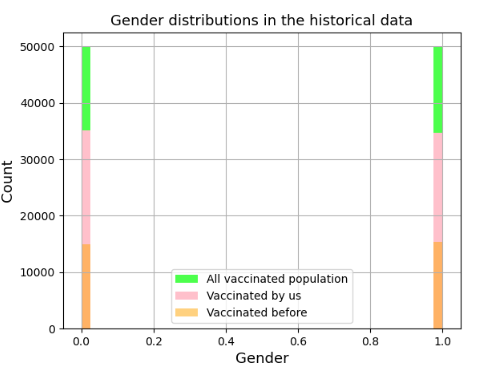
\includegraphics[height=6cm]{hd_gender_dist_version2.png}
    \caption{Gender distribution in the historical data after $10$ vaccination stages.}
    \label{hd_gender_dist}
\end{figure}


In \textbf{Figure \ref{hd_gender_dist}} we see that the distribution of men and women in our collected data is roughly half and half for each gender, which is in line with our expectation. From this standpoint we can say that the starting data is fairly collected with respect to $Gender$.

Next, we look at the age variable in the data. In contrast to $Gender$, the $Age$ variable is a floating point number in a range from 0 to roughly 100. For this reason we analyze the Ages of the population in "buckets", where we count the number of people in sub-ranges of ages, which is to say how many people are of an age between certain numbers ($0-30$, $30-60$, etc.). This distribution is not expected to be completely uniform, as a consequence of human mortality implying  that there will be fewer individuals above the age of $80$ than above $70$. Nonetheless, in order to find that the data is collected fairly, we should expect that each age group will be represented sufficiently to make informed decisions with their data. \textbf{Figure \ref{hd_age_dist}} shows the distribution of ages (not bucketed) in the initial data, showing a distribution with an average near $25$ and declining towards $100$ (with some examples well above $100$ which we might attribute to data entry error). This distribution reflects a relatively young population, but nonetheless is generally in line with what we might expect from a "population pyramid" with declining numbers of elderly individuals. Importantly we see sufficient numbers of data points for these individuals to be able to make reasonably informed decisions with a machine learning algorithm.

\begin{figure}[H]
    \centering
    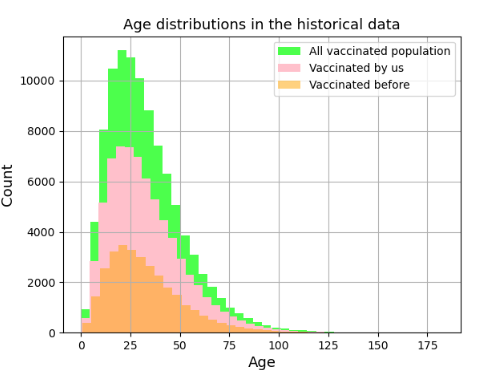
\includegraphics[height=6cm]{hd_age_dist_version2.png}
    \caption{Age distribution in the historical data after $10$ vaccination stages.}
    \label{hd_age_dist}
\end{figure}


Lastly, we analyze the $Income$ variable of the data to assess the distribution of incomes among the population. Here we expect that an unfairly collected set of data might be unreasonably skewed towards higher income, as oftentimes higher income individuals may have better access to healthcare and ability to take part in treatment programs. It is for this reason crucial that we appropriately collect data from low-income members of the population such that the vaccination decisions we take are not biased to give preferential outcomes according to income.

\begin{figure}[H]
    \centering
    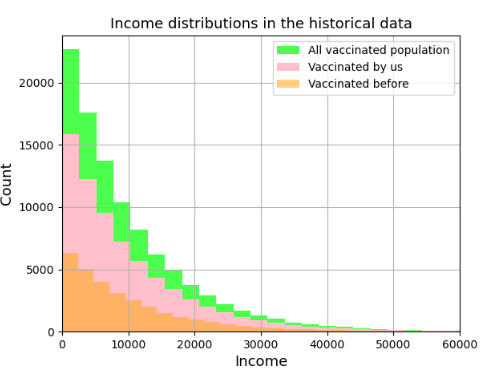
\includegraphics[height=6cm]{hd_income_dist_version2.png}
    \caption{Income distribution in the historical data after $10$ vaccination stages.}
    \label{hd_income_dist}
\end{figure}

\textbf{Figure \ref{hd_income_dist}} shows that the $Income$ variable in the data follows a power law distribution in which the largest chunk of individuals have no or little income, declining towards $0$ individuals as income increases. This kind of observation is discussed extensively in economics literature \textcolor{blue}{\cite{gabaix2016power}} and it is therefore unsurprising that comparatively few individuals make the highest incomes. For the same reason it appears appropriate to conclude that the data collection was not biased towards collection of higher income individuals' data, but also represents them to the degree that we would expect.

%We look at the amount of each group in the data and see if the incomes are in line with actual income distributions in the general population and if the data is representative of that with respect to income, age, gender.
%We also look at which groups get vaccinated and whether the rates of vaccination between them are different.

%We also analyze our decision making function and look at the outcomes and see how fair they are. We find that they are (fair|unfair) because our analysis shows this.

\section{Analyzing the Data \& Outcomes in Decision Making}

Following from our initial analysis of the data and its collection, we then look to investigate fairness as we make use of it for our decision making. As stated previously, we are attempting to design (or more specifically, train a machine learning model to produce) a vaccination policy which will result in the lowest number of deaths in the population. In the interest of fairness, we must look at the outcomes of this policy with respect to the sensitive variables identified in the previous section. An overview of this investigation can be demonstrated in the tables below. We look at the outcomes in three different cases: Among the previously vaccinated population (those with vaccines prior to our policy), among those vaccinated as a result of our policy, and the overall numbers among the whole vaccinated population

%Adding simple histograms and visualization of outcomes here.
%Can talk about how our model only uses the selected features so it isn't ever selecting age gender or income but instead comorbidities and genes to make decisions with. So this means we're not using the sensitive features.

At a general level, we observe that our policy results in outcomes that are in line with the original trends of the data, which is to say that our policy does not disproportionately improve the outcome of one group relative to another when considering the sensitive variables. In the cases of the previously vaccinated population as well as the population we vaccinate, the probability of both receiving a specific vaccine (chance of action) and the probability of death (chance of outcome) are nearly equal across all groups of $Age$, $Gender$, and $Income$. One possible reason for the fair outcomes we observe from our policy is that our model is trained only using the top predictive features of death, which have in all cases been genes and comorbidities. Age is the most likely feature that we would expect to be predictive, but it has not been used in the models. While forgoing the use of sensitive variables in training a model is not in itself sufficient to guarantee fairness, in this case we suspect it may be enough to prevent unfair outcomes. It is also for this reason that, while it would be possible to design a utility function which balances fairness and raw utility e.g. a loss function $\mathcal{L}(U) = U + F(U)$ where we optimize via Stochastic Gradient Descent, in the case of our policy the observed outcomes suggest such an approach would be unnecessary.

%We can also describe the theory of SGD and fairness and why we don't need to use it since the outcomes seem to already be fair

\section{Calibration of Outcome When the Sensitive Variable Differs}

As mentioned in \textbf{Section \ref{sec: Calibration}} it is also instructive for us to look at the \textit{Calibration} of the policy with respect to the sensitive variables. First, we calculate the probability of an action given a sensitive variable (in accordance with the notions of fairness described in \textbf{Section \ref{sec: Introduction}}). We then measure the calibration of our decision making algorithm by analyzing the variation in the outcome with respect to the identified variables. This probability is calculated as described in \textbf{Section \ref{sec: Calibration}}.

Therefore, in this part of our analysis we calculate the conditional probabilities of both the outcomes and actions taken both in the original data and as a result of our policy. We wish to discover whether any discrepancies exist between groups in terms of either receiving certain vaccines or the risk of death in the data. 


%% for all vaccinated population
\begin{center}
\begin{table}[H]
\begin{adjustbox}{max width=\textwidth}
\begin{tabular}{ |c| c c c c c c c| }
\hline
A  & \multicolumn{7}{c|}{Z} \\
\hline
  & Age$\leq30$ &    $30<$Age$<60$ &     Age$\geq60$ &    Female &      Male &   $0k\leq$Income$<10k$ &    Income$\geq10k$ \\
\hline
 Vaccine1 & 0.344259 &  0.340701 &  0.333370 &  0.343092 &  0.340631 &  0.344769 &  0.336853 \\ 
 Vaccine2 &  0.329845 &  0.334998 &  0.340153 &  0.331898 &  0.333740 &  0.331362 &  0.335329 \\  
 Vaccine3 & 0.325896 &  0.324302 &  0.326477 &  0.325010 &  0.325629 &  0.323869 &  0.327818  
 \\ \hline
\end{tabular}
\end{adjustbox}
\caption{Table containing values of $\mathbb{P}(a|z)$ for '\textit{all vaccinated population}' space.}
\label{tab:1}
\end{table}
\end{center}


%% for vaccinated by us
\begin{center}
\begin{table}[H]
\begin{adjustbox}{max width=\textwidth}
\begin{tabular}{ |c| c c c c c c c|}
\hline
A  & \multicolumn{7}{c|}{Z} \\
\hline
  & Age$\leq30$ &    $30<$Age$<60$ &     Age$\geq60$ &    Female &      Male &   $0k\leq$Income$<10k$ &    Income$\geq10k$ \\
\hline
 Vaccine1 &  0.351686 &  0.342963 &  0.330376 &  0.346957 &  0.345681 &  0.351249 &  0.337800 \\
 Vaccine2 & 0.327493 &  0.334581 &  0.349390 &  0.332307 &  0.332224 &  0.330389 &  0.335508 \\  
 Vaccine3 &  0.320822 &  0.322456 &  0.320235 &  0.320735 &  0.322095 &  0.318363 &  0.326692  
  \\ \hline
\end{tabular}
\end{adjustbox}
\caption{Table containing values of $\mathbb{P}(a|z)$ for '\textit{vaccinated by us}' space.}
\label{tab:2}
\end{table}
\end{center}




%% for vaccinated before
\begin{center}
\begin{table}[H]
\begin{adjustbox}{max width=\textwidth}
\begin{tabular}{ |c| c c c c c c c|}
\hline
A  & \multicolumn{7}{c|}{Z} \\
\hline
  & Age$\leq30$ &    $30<$Age$<60$ &     Age$\geq60$ &    Female &      Male &   $0k\leq$Income$<10k$ &    Income$\geq10k$ \\
\hline
 Vaccine1 &  0.326702 &  0.335306 &  0.340049 &  0.333962 &  0.328729 &  0.329408 &  0.334636 \\
 Vaccine2 &  0.335406 &  0.335992 &  0.319548 &  0.330932 &  0.337312 &  0.333671 &  0.334909 \\
 Vaccine3 &  0.337893 &  0.328701 &  0.340403 &  0.335106 &  0.333959 &  0.336921 &  0.330455
  \\ \hline
\end{tabular}
\end{adjustbox}
\caption{Table containing values of $\mathbb{P}(a|z)$ for '\textit{vaccinated before}' space.}
\label{tab:3}
\end{table}
\end{center}

In \textbf{Tables \ref{tab:1}, \ref{tab:2}, \ref{tab:3}}, we observe the probability of actions taken dependent on the demographic groups. This is to say that each cell value describes the chance that a member of the column group will receive the vaccine in the row label. Overall, the vaccines are generally evenly distributed among the groups in the previously vaccinated population, as well as among the population our policy chooses to vaccinate. There is a slight preference for vaccination with $Vaccine1$ under our policy whereas in the original data no vaccine is more likely than the others for any group. However, for the purposes of fairness our policy succeeds in that this preference for choosing $Vaccine1$ applies to all demographic groups with the one exception of those at or above the age of $60$. The difference for this group does not in itself indicate the policy is overall unfair, because as state previously there may be a valid reason such as $Vaccine2$ working more effectively in preventing death in this group.

\begin{center}
    \begin{table}[H]
    \centering
        \begin{tabular}{ |c| c c c|}
            \hline
            & Vaccine1 &  Vaccine2 & Vaccine3  \\
            \hline
            All population & 0.341860 &  0.332820 &  0.325320 \\
            Vaccinated by us  &  0.346319 &  0.332265 &  0.321416 \\
            Vaccinated before &  0.331340 &  0.334128 &  0.334532
            \\ \hline
        \end{tabular}
    \caption{Table containing values of $\mathbb{P}(a)$ for all spaces (subsets).}
    \label{tab:Pa_summary}
    \end{table}    
\end{center}

\textbf{Table \ref{tab:Pa_summary}} summarizes the overall probability of receiving each vaccine among the population. Following the intuition behind equation (\ref{eq: 1}), \tetxbf{Table \ref{tab:Pa_summary}} should express the probability of outcomes given a fair policy, and subsequently we should observe \textbf{Tables \ref{tab:1}, \ref{tab:2} and \ref{tab:3}} displaying equivalent probabilities for each group (this is to say that no group has a disparate outcome when compared to the overall outcomes).

Next we investigate the \textit{outcomes} of the vaccinations. This analysis relates to the $Calibration$ of the policy as mentioned before (\textbf{Section} \ref{sec: Calibration}), and we are calculating the probability of death given an action and a sensitive variable. Analysis of this data is then summarized by three sets of three tables, where the sets of tables describe outcomes of the overall vaccination, our vaccination, and previous vaccination, respectively. Each set contains a table describing the overall probability of death in that population, one describing the conditional probability of death given an action and demographic group, and a table showing the difference in outcome for a group compared to the overall outcome.

% calibration
% table for all population space
% $\mathbb{P}(y | a)$
\begin{center}
    \begin{table}[H]
    \centering
        \begin{tabular}{ |c| c c c|}
            \hline
            & Vaccine1 &  Vaccine2 & Vaccine3  \\
            \hline
            Dead &  0.004359 &  0.004837 &  0.005379
            \\ \hline
        \end{tabular}
    \caption{Table containing $\mathbb{P}(y | a)$ for '\textit{all vaccinated population}' space.}
    \label{tab:simple_prob_py_a}
    \end{table}
\end{center}

%\textbf{Table \ref{tab:simple_prob_py_a}} describes the overall probability of death given an action ($Vaccine$) among the population. This simple metric gives us the indication that among the population as a whole, $Vaccine3$ is less effective in preventing death. The probability of death is approximately $0.001\%$ higher than $Vaccine1$, and $0.0005\%$  higher than $Vaccine2$. As $Vaccine1$ appears to be the most effective in preventing death, this is the vaccine that our policy learns to apply most frequently.

%Finally, \textbf{tables \ref{tab:6}, \ref{tab:8}, and \ref{tab:10}} show the probability of the outcome "death" given both the action and the sensitive variable. Here we are investigating the outcomes when broken down by demographic group. We compare these numbers with the overall probability of death in order to determine whether certain groups have outcomes worse than the overall probability.

% calibration
% table for all population space
% $\mathbb{P}(y | az)$
\begin{center}
\begin{table}[H]
\begin{adjustbox}{max width=\textwidth}
    \begin{tabular}{ |c| c c c c c c c|}
        \hline
          A  & \multicolumn{7}{c|}{Z} \\
          \hline
          & Age$\leq30$ &    $30<$Age$<60$ &     Age$\geq60$ &    Female &      Male &   $0k\leq$Income$<10k$ &    Income$\geq10k$  \\
        \hline
        Vaccine1 &  0.004521 &  0.004092 &  0.004595 &  0.004377 &  0.004340 &  0.004173 &  0.004686 \\
        Vaccine2 &  0.004246 &  0.005750 &  0.004181 &  0.004646 &  0.005028 &  0.004628 &  0.005194 \\
        Vaccine3 &  0.005253 &  0.005862 &  0.004021 &  0.005237 &  0.005521 &  0.005662 &  0.004898
         \\ \hline
    \end{tabular}
    \end{adjustbox}
    \caption{Table containing $\mathbb{P}(y | a, z)$ for '\textit{all vaccinated population}' space.}
    \label{tab:6}
\end{table}
\end{center}

\begin{center}
\begin{table}[H]
\begin{adjustbox}{max width=\textwidth}
    \begin{tabular}{ |c| c c c c c c c|}
        \hline
          A  & \multicolumn{7}{c|}{Z} \\
          \hline
          & Age$\leq30$ &    $30<$Age$<60$ &     Age$\geq60$ &    Female &      Male &   $0k\leq$Income$<10k$ &    Income$\geq10k$  \\
        \hline
        Vaccine1 &  0.000162 &  0.000267 &  0.000236 &  0.000018 &  0.000019 &  0.000186 &  0.000327 \\
        Vaccine2 &  0.000591 &  0.000913 &  0.000656 &  0.000191 &  0.000191 &  0.000209 &  0.000357 \\
        Vaccine3 &  0.000126 &  0.000483 &  \textbf{\textcolor{red}{0.001358}} &  0.000142 &  0.000142 &  0.000283 &  0.000481
         \\ \hline
    \end{tabular}
    \end{adjustbox}
    \caption{Table containing $| \mathbb{P}(y | a, z) - \mathbb{P}(y | a) |$ for '\textit{all vaccinated population}' space.}
    \label{tab:diff}
\end{table}
\end{center}

In \textbf{Tables \ref{tab:simple_prob_py_a} and \ref{tab:6}}, we apply the formula for calibration (\ref{eq: Calibration}) and obtain the conditional probabilities describing first the overall probability of death when given a vaccine, and secondly the probability of death given a vaccine and a sensitive attribute. Our goal here is to compare the demographic specific chances of death to the overall value, so that we can identify any groups which may have a disproportionately large risk of death relative to others. If there is no identifiable or substantial difference between the table values, then we can infer that the outcomes of the policy are fair.

Comparing \textbf{Table \ref{tab:6} to Table \ref{tab:simple_prob_py_a}}, we can then summarize the results as in \textbf{Table \ref{tab:diff}}. Here we can observe the difference between each group's outcome and the overall outcome (probability of death). We can see that the highest disparity is among the most elderly ($60$ or older) who received $Vaccine3$. In this group, the chance of death was approximately $0.001\%$ higher than the overall chance of death. The next largest disparity is in outcomes for people between the ages of $30$ and $60$ who have been given $Vaccine2$. The chance of death for this group is nearly $0.001\%$ higher than the average value, indicating that this group is also likely to be affected unfavorably by any decisions to give them $Vaccine2$. Subsequently, the next highest values are among the other two age groups when they received $Vaccine2$, indicating that $Vaccine2$ provides a worse outcome when evaluating the results with respect to age. In any case, none of these values are especially large, so they do not indicate that the decisions of previous or current vaccination policy are grossly unfair to this group. All other deviations from the overall probability of death are negligible, and from this we have an indication that the policy is fair with respect to beneficial outcomes (survival).

% calibration
% table for vaccinated by us
% $\mathbb{P}(y | a)$
\begin{center}
\begin{table}[H]
\centering
    \begin{tabular}{ |c| c c c|}
    \hline
      & Vaccine1 &  Vaccine2 & Vaccine3  \\
    \hline
    Dead &  0.004522 &  0.004928 &   0.00567
     \\ \hline
    \end{tabular}
%\caption{Probability of death among recipients of each vaccine from our policy}
    \caption{Table containing $\mathbb{P}(y | a)$ for '\textit{vaccinated by us}' space.}
\end{table}
\end{center}

% calibration
% table for vaccinated by us
% $\mathbb{P}(y | az)$
\begin{center}
    \begin{table}[H]
    \begin{adjustbox}{max width=\textwidth}
        \begin{tabular}{ |c| c c c c c c c|}
            \hline
              A  & \multicolumn{7}{c|}{Z} \\
              \hline
              & Age$\leq30$ &    $30<$Age$<60$ &     Age$\geq60$ &    Female &      Male &   $0k\leq$Income$<10k$ &    Income$\geq10k$ \\
            \hline
            Vaccine1 &  0.004801 &  0.004196 &  0.004317 &  0.005258 &  0.003786 &  0.004224 &  0.005059 \\
            Vaccine2 &  0.004057 &  0.006237 &  0.004082 &  0.004546 &  0.005310 &  0.004422 &  0.005788 \\
            Vaccine3 &  0.005608 &  0.005802 &  0.005443 &  0.005421 &  0.005918 &  0.005931 &  0.005231 
             \\ \hline
        \end{tabular}
        \end{adjustbox}
        \caption{Table containing $\mathbb{P}(y | a, z)$ for '\textit{vaccinated by us}' space.}
        \label{tab:8}
    \end{table}
\end{center}


\begin{center}
\begin{table}[H]
\begin{adjustbox}{max width=\textwidth}
    \begin{tabular}{ |c| c c c c c c c|}
        \hline
          A  & \multicolumn{7}{c|}{Z} \\
          \hline
          & Age$\leq30$ &    $30<$Age$<60$ &     Age$\geq60$ &    Female &      Male &   $0k\leq$Income$<10k$ &    Income$\geq10k$  \\
        \hline
        Vaccine1 &  0.000279 &  0.000326 &  0.000205 &  0.000736 &  0.000736 &  0.000298 &  0.000537 \\
        Vaccine2 &  0.000871 &  \textbf{\textcolor{red}{0.001309}} &  0.000846 &  0.000382 &  0.000382 &  0.000506 &  0.000860 \\
        Vaccine3 &  0.000062 &  0.000132 &  0.000227 &  0.000249 &  0.000248 &  0.000261 &  0.000439
         \\ \hline
    \end{tabular}
    \end{adjustbox}
    \caption{Table containing $| \mathbb{P}(y | a, z) - \mathbb{P}(y | a) |$ for '\textit{vaccinated by us}' space.}
    \label{tab:diff1}
\end{table}
\end{center}

We can continue this analysis on the level of the population whom we have vaccinate with our policy. Again we seek to uncover any disparities in the chance of death given a vaccine for each population, this time restricting ourselves to analyzing those individuals whose outcomes are a consequence of the actions we have taken. This is perhaps the most important group to look at in this way, because these are the results that are within our control as designers of the vaccination policy.

In \textbf{Table \ref{tab:diff1}} we summarize the difference in outcome per group versus the overall outcomes in the same manner as before. For this group, we observe the age group between $30$ and $60$ years old given $Vaccine2$ had the largest difference in outcome from the overall probability, at approximately $0.001\%$ (similarly to before). Overall, the values are somewhat higher than among the overall population, but they are again very low and there are not substantial differences in outcomes for specific groups. One very interesting result that is also shown in this table is that the outcomes between males and females are identical in the case of $Vaccines$ $1$ and $2$, and nearly so in the case of $Vaccine3$. Additionally, when comparing to \textbf{Tables \ref{tab:pya vaccinated before} and \ref{tab:pyaz vaccinated before}} (further below), we observe that our policy has improved the outcomes for the lower income population at the cost of somewhat worsened outcomes for those with incomes above $10k$. At face value, this appears to swap outcomes between groups for no apparent advantage, however when we consider that as shown in \textbf{Figure \ref{hd_income_dist}}, by far the largest segment of the population is low income. In this regard, our policy represents an improvement in that the outcomes for a larger segment of the population are improved.

% calibration
% table for vaccinated before
% $\mathbb{P}(y | a)$
\begin{center}
    \begin{table}[H]
    \centering
        \begin{tabular}{ |c| c c c|}
            \hline
            & Vaccine1 &  Vaccine2 & Vaccine3  \\
            \hline
            Dead &  0.003954 &  0.004625 &   0.00472
            \\ \hline
        \end{tabular}
    \caption{Table containing $\mathbb{P}(y | a)$ for '\textit{vaccinated before}' space.}
    \label{tab:pya vaccinated before}
    \end{table}
\end{center}

% calibration
% table for vaccinated before
% $\mathbb{P}(y | az)$
\begin{center}
    \begin{table}[H]
    \begin{adjustbox}{max width=\textwidth}
        \begin{tabular}{ |c| c c c c c c c|}
            \hline
            A  & \multicolumn{7}{c|}{Z} \\
            \hline
            & Age$\leq30$ &    $30<$Age$<60$ &     Age$\geq60$ &    Female &      Male &   $0k\leq$Income$<10k$ &    Income$\geq10k$  \\
            \hline
            Vaccine1 &  0.003806 &  0.003837 &  0.005198 &  0.002217 &  0.005712 &  0.004044 &  0.003803 \\
            Vaccine2 &  0.004683 &  0.004595 &  0.004425 &  0.004882 &  0.004374 &  0.005110 &  0.003800 \\
            Vaccine3 &  0.004455 &  0.006002 &  0.001038 &  0.004821 &  0.004618 &  0.005061 &  0.004127 
            \\ \hline
        \end{tabular}
        \end{adjustbox}
    \caption{Table containing $\mathbb{P}(y | a, z)$ for '\textit{vaccinated before}' space.}
    \label{tab:pyaz vaccinated before}
    \end{table}
\end{center}

\begin{center}
\begin{table}[H]
\begin{adjustbox}{max width=\textwidth}
    \begin{tabular}{ |c| c c c c c c c|}
        \hline
          A  & \multicolumn{7}{c|}{Z} \\
          \hline
          & Age$\leq30$ &    $30<$Age$<60$ &     Age$\geq60$ &    Female &      Male &   $0k\leq$Income$<10k$ &    Income$\geq10k$  \\
        \hline
        Vaccine1 &  0.000162 &  0.000267 &  0.000236 &  0.000018 &  0.000019 &  0.000186 &  0.000327 \\
        Vaccine2 &  0.000591 &  0.000913 &  0.000656 &  0.000191 &  0.000191 &  0.000209 &  0.000357 \\
        Vaccine3 &  0.000126 &  0.000483 &  \textbf{\textcolor{red}{0.001358}} &  0.000142 &  0.000142 &  0.000283 &  0.000481
         \\ \hline
    \end{tabular}
    \end{adjustbox}
    \caption{Table containing $| \mathbb{P}(y | a, z) - \mathbb{P}(y | a) |$ for '\textit{vaccinated before}' space.}
    \label{tab:diff2}
\end{table}
\end{center}

For the purpose of comparison and to investigate the fairness of vaccination decisions made prior to our policy, we perform the same analysis on the previously vaccinated individuals in the data. As mentioned previously, we can compare the outcomes among income groups and conclude that the previously vaccinated population displayed slightly better outcomes for those with income above $10k$. In this group, the largest difference in outcome was observed in the $60$ or older age group who received $Vaccine3$, once again at approximately $0.001\%$ difference. The previous policy was also not especially unfair, as the differences in chance of death were not massively disparate. The same finding of similar to identical outcomes among men and women also applies to the previously vaccinated population. This feature of the data may indicate that our policy was able to learn from the prior vaccinations in a way that preserved this aspect of fairness in vaccination with respect to gender.

\section{Unifying view of fairness and Conclusion}
\label{sec: Conclusion}

Finally, we take a "unifying" view of fairness with which to investigate the policy, in that we want to measure any disparities in outcomes when measuring the calibration of the policy. This unifying measure of fairness with respect to the policy is defined (see \textcolor{blue}{\cite{Dimitrakakis}}) as follows:

\begin{equation}
\label{eq: F_calibration}
    \mathcal{F}_{\text{Calibration}}(\theta, \pi) \triangleq \max_{a, z} \sum_{i} \bigg{|}\mathbb{P}_{\theta}^{\pi}(y=i|a,z) - \mathbb{P}_{\theta}^{\pi}(y=i|a,z^{\prime})\bigg{|}
\end{equation}

This is, we evaluate the difference in outcomes between different values of sensitive attributes and select the largest absolute value of the difference. Our measure here gives an indication of how large the disparity in outcomes between different groups may be, where a larger difference indicates greater disparity. In the following tables, we summarize the $F$ values that we calculate over our policy for the sensitive variables we identified. This is as before broken down into the entire vaccinated population, the population vaccinated by our policy, and the previously vaccinated population, respectively.

\begin{table}[H]
    \begin{adjustbox}{max width=\textwidth}
        \begin{tabular}{|c| c c c c c c c|}
        \hline
          & Age$\leq30$ &    $30<$Age$<60$ &     Age$\geq60$ &    Female &      Male &   $0k\leq$Income$<10k$ &    Income$\geq10k$  \\
        \hline
         Age$\leq30$ & 0.000000 &  0.001504 &  0.001232 &  0.000400 &  0.000782 &  0.000409 &  0.000948 \\
        \hline
        $30<$Age$<60$ &  0.001504 &  0.000000 &  \textbf{\textcolor{red}{0.001841}} &  0.001104 &  0.000722 &  0.001122 &  0.000964 \\
        \hline
        Age$\geq60$ &  0.001232 &  \textbf{\textcolor{red}{0.001841}} &  0.000000 &  0.001216 &  0.001500 &  0.001641 &  0.001013 \\
        \hline
        Female &  0.000400 &  0.001104 &  0.001216 &  0.000000 &  0.000382 &  0.000425 &  0.000548 \\
        \hline
        Male &  0.000782 &  0.000722 &  0.001500 &  0.000382 &  0.000000 &  0.000400 &  0.000623 \\
        \hline
        $0k\leq$Income$<10k$ &  0.000409 &  0.001122 &  0.001641 &  0.000425 &  0.000400 &  0.000000 &  0.000764 \\
        \hline
        Income$\geq10k$ &  0.000948 &  0.000964 &  0.001013 &  0.000548 &  0.000623 &  0.000764 &  0.000000 
        \\ \hline
        \end{tabular}
    \end{adjustbox}
\caption{Table containing the $\mathcal{F}_{\text{calibration}}$'s values for our sensitive variables $z$ for '\textit{all vaccinated population}' space.}
\label{tab:14}
\end{table}


\begin{center}
\begin{table}[H]
\begin{adjustbox}{max width=\textwidth}
    \begin{tabular}{ |c| c c c c c c c|}
    \hline
      & Age$\leq30$ &    $30<$Age$<60$ &     Age$\geq60$ &    Female &      Male &   $0k\leq$Income$<10k$ &    Income$\geq10k$  \\
    \hline
     Age$\leq30$ &  0.000000 &  \textbf{\textcolor{red}{0.002180}} &  0.000484 &  0.000489 &  0.001253 &  0.000577 &  0.001731 \\
    \hline
    $30<$Age$<60$ &  \textbf{\textcolor{red}{0.002180}} &  0.000000 &  0.002155 &  0.001691 &  0.000927 &  0.001815 &  0.000863 \\
    \hline
    Age$\geq60$ &  0.000484 &  0.002155 &  0.000000 &  0.000941 &  0.001228 &  0.000488 &  0.001706 \\
    \hline
    Female &  0.000489 &  0.001691 &  0.000941 &  0.000000 &  0.001472 &  0.001034 &  0.001242 \\
    \hline
    Male &  0.001253 &  0.000927 &  0.001228 &  0.001472 &  0.000000 &  0.000888 &  0.001273 \\
    \hline
    $0k\leq$Income$<10k$ &  0.000577 &  0.001815 &  0.000488 &  0.001034 &  0.000888 &  0.000000 &  0.001366 \\
    \hline
    Income$\geq10k$ &  0.001731 &  0.000863 &  0.001706 &  0.001242 &  0.001273 &  0.001366 &  0.000000 
    \\ \hline
    \end{tabular}
    \end{adjustbox}
\caption{Table containing the $\mathcal{F}_{\text{calibration}}$'s values for our sensitive variables $z$ for '\textit{vaccinated by us}' space.}
\label{tab:15}
\end{table}
\end{center}


\begin{center}
\begin{table}[H]
\begin{adjustbox}{max width=\textwidth}
    \begin{tabular}{ |c| c c c c c c c|}
    \hline
      & Age$\leq30$ &    $30<$Age$<60$ &     Age$\geq60$ &    Female &      Male &   $0k\leq$Income$<10k$ &    Income$\geq10k$  \\
    \hline
     Age$\leq30$ &  0.000000 &  0.001547 &  0.003417 &  0.001589 &  0.001906 &  0.000606 &  0.000883 \\
    \hline
    $30<$Age$<60$ &  0.001547 &  0.000000 &  \textbf{\textcolor{red}{0.004964}} &  0.001620 &  0.001875 &  0.000941 &  0.001875 \\
    \hline
    Age$\geq60$ &  0.003417 &  \textbf{\textcolor{red}{0.004964}} &  0.000000 &  0.003783 &  0.003580 &  0.004023 &  0.003089 \\
    \hline
    Female &  0.001589 &  0.001620 &  0.003783 &  0.000000 &  0.003495 &  0.001827 &  0.001586 \\
    \hline
    Male &  0.001906 &  0.001875 &  0.003580 &  0.003495 &  0.000000 &  0.001668 &  0.001909 \\
    \hline
    $0k\leq$Income$<10k$ &  0.000606 &  0.000941 &  0.004023 &  0.001827 &  0.001668 &  0.000000 &  0.001310 \\
    \hline
    Income$\geq10k$ &  0.000883 &  0.001875 &  0.003089 &  0.001586 &  0.001909 &  0.001310 &  0.000000 
    \\ \hline
    \end{tabular}
    \end{adjustbox}
\caption{Table containing the $\mathcal{F}_{\text{calibration}}$'s values for our sensitive variables $z$ for '\textit{vaccinated before}' space.}
\label{tab:16}
\end{table}
\end{center}

We first observe that among the general population of vaccinated individuals, the greatest dispararity in outcome with respect to our measure in this section is between those who are $60$ years or older and those between $30$ and $60$ years old, with a difference of almost $0.002\%$. What this says intuitively is that the difference in outcomes is greatest between these two groups when observing the entire vaccinated population. We can then compare this and other values in this table with \textbf{Table \ref{tab:15}}, which displays the same measure when calculated within the population of individuals vaccinated under our policy. In this case, the greatest difference is between those aged $30$ years or less and those between $30$ and $60$ years old, again with a value of approximately $0.002\%$. The final table, \textbf{Table \ref{tab:16}}, displays the previous policy results, where the greatest difference again lies between the oldest and middle age group, standing with a difference of nearly $0.005\%$. This is over twice the greatest difference in outcomes observed in the results of our policy, providing a good indication that our policy presents a substantial improvement in fairness when we evaluate outcomes by comparing group outcomes to one another. This is a more granular view of the issue and allows us to reason more specifically about why a policy could be considered fair, in that by fairness we somewhat inherently must be comparing between groups, rather than absolute values in outcomes. For this reason, despite the earlier analysis being somewhat inconclusive in determining whether previous policy or our policy is more fair (with the caveat that both are broadly fair in absolute terms), we can say in conclusion that our policy appears to make fairer decisions which result in less disparate outcomes for the population.

\addcontentsline{toc}{section}{References}
\printbibliography
\end{document}
